\documentclass[aspectratio=169, 10pt]{beamer}

% --- Theme and Visual Setup ---
\usetheme{metropolis}
\metroset{
  progressbar=frametitle,
  block=fill,
  titleformat frame=regular
}

% --- Packages ---
\usepackage{graphicx}
\usepackage{booktabs}
\usepackage{tabularx}
\usepackage{makecell}
\usepackage{xcolor}
\usepackage{subcaption}
\usepackage{colortbl}

% --- Custom Colors & Visual Styling ---
\definecolor{darkblue}{RGB}{20, 40, 80}
\definecolor{tealaccent}{RGB}{0, 128, 128}
\definecolor{lightgraybg}{RGB}{245, 247, 250}

\setbeamercolor{frametitle}{fg=white, bg=darkblue}
\setbeamercolor{progress bar}{fg=tealaccent, bg=gray!30}
\setbeamercolor{alerted text}{fg=tealaccent}
\setbeamercolor{block title}{fg=white, bg=darkblue}
\setbeamercolor{block body}{fg=black, bg=lightgraybg}

% --- Metadata ---
\title[ReXGroundingCT 3D Data Profiling]{ReXGroundingCT 3D Data Profiling, Spatial Priors \& Prompt Syntax}
\subtitle{MICCAI 2026 Challenge Benchmark Investigation}
\author{ReXGroundingCT Challenge Research Team}
\date{July 28, 2026}

\begin{document}

% ==============================================================================
% SLIDE 1: Title
% ==============================================================================
\begin{frame}
    \titlepage
\end{frame}

% ==============================================================================
% SLIDE 2: Dataset Hierarchy
% ==============================================================================
\begin{frame}{Dataset Indexing Hierarchy}
    \vspace{-0.5em}
    \begin{block}{Tier 1: Physical NIfTI Scans (3,078 Volumes)}
        \footnotesize 2,578 Train / 200 Val / 300 Test physical scan acquisition sessions.
    \end{block}
    
    \vspace{-0.3em}
    \centering \tiny \color{tealaccent} $\downarrow$ Multi-kernel series indexing (\texttt{\_1.nii.gz}, \texttt{\_2.nii.gz}) \color{black}
    \vspace{-0.3em}
    
    \begin{block}{Tier 2: Dataset Record Entries (3,192 Records)}
        \footnotesize 2,992 Train / 200 Val indexed entries in \texttt{dataset.json} (with raw reports).
    \end{block}
    
    \vspace{-0.3em}
    \centering \tiny \color{tealaccent} $\downarrow$ GPT-4 parses raw reports into discrete finding text queries \color{black}
    \vspace{-0.3em}
    
    \begin{block}{Tier 3: Report Prompts (8,650 Free-Text Queries)}
        \footnotesize 8,650 radiology sentence prompts (81.4\% unique verbatim text).
    \end{block}
    
    \vspace{-0.3em}
    \centering \tiny \color{tealaccent} $\downarrow$ Radiologists segment 3D voxel masks paired to each text query \color{black}
    \vspace{-0.3em}
    
    \begin{block}{Tier 4: Target Finding Masks (8,650 3D Masks)}
        \footnotesize 7,687 Train (Entity protocol $\le 3$) / 381 Val (Exhaustive) / 582 Test 3D segmentation masks.
    \end{block}
\end{frame}

% ==============================================================================
% SLIDE 3: Table 1 - Dataset Split Overview & Disparity
% ==============================================================================
\begin{frame}{Table 1: Dataset Split Overview \& Disparity}
    \centering
    \small
    \begin{tabular}{lcccccc}
        \toprule
        \textbf{Split} & \makecell{\textbf{Records /}\\\textbf{Physical Scans}} & \textbf{Findings} & \makecell{\textbf{Findings}\\\textbf{/ Record}} & \makecell{\textbf{Mean Inst}\\\textbf{/ Finding}} & \textbf{Std Inst} & \textbf{Max Inst} \\
        \midrule
        \textbf{Train} & 2,992 (2,578) & 7,687 & 2.57 & 1.948 & $\pm 0.962$ & 11 \\
        \textbf{Val}   & 200 (200)     & 381   & 1.91 & \textbf{3.714} & $\pm 4.441$ & \textbf{36} \\
        \textbf{Test}  & 300 (300)     & 582   & 1.94 & 1.000 & $\pm 0.000$ & 1 \\
        \bottomrule
    \end{tabular}

    \vspace{1.5em}
    \begin{columns}[c]
        \begin{column}{0.95\textwidth}
            \begin{itemize}
                \item \textbf{Train Protocol:} Entity Protocol capping annotated instances ($\le 3$ per finding query).
                \item \textbf{Val Protocol:} Exhaustive annotation of all visible instances ($1.91\times$ quantitative disparity).
            \end{itemize}
        \end{column}
    \end{columns}
\end{frame}

% ==============================================================================
% SLIDE 4: Table 2 - 14-Category Breakdown
% ==============================================================================
\begin{frame}{Table 2: 14-Category Breakdown \& Disparity Ratios}
    \centering
    \tiny
    \setlength{\tabcolsep}{4pt}
    \begin{tabular}{clccccc}
        \toprule
        \textbf{Code} & \textbf{Category Name} & \textbf{Type} & \textbf{Train Prev (\%)} & \textbf{Val Prev (\%)} & \textbf{Train Mean Inst.} & \textbf{Val Mean Inst.} & \textbf{Disparity Ratio} \\
        \midrule
        \texttt{1a} & Bronchial wall thickening & Non-Focal & 7.09 & 1.50 & 2.05 & 4.00 & 1.95x \\
        \texttt{1b} & Bronchiectasis           & Non-Focal & 8.26 & 4.50 & 2.10 & 3.27 & 1.56x \\
        \texttt{1c} & Emphysema                & Non-Focal & 13.97 & 7.50 & 2.39 & 2.82 & 1.18x \\
        \texttt{1d} & Septal thickening        & Non-Focal & 6.15 & 3.00 & 2.22 & 5.50 & 2.48x \\
        \texttt{1e} & Micronodules             & Non-Focal & 7.99 & 5.50 & 2.21 & 5.18 & 2.35x \\
        \texttt{1f} & Other non-focal          & Non-Focal & 4.75 & 2.00 & 2.08 & 2.75 & 1.32x \\
        \midrule
        \texttt{2a} & Linear opacities         & Focal & 26.77 & 31.50 & 1.71 & 2.25 & 1.31x \\
        \texttt{2b} & Atelectasis / consolid.  & Focal & 30.45 & 20.00 & 1.78 & 2.78 & 1.56x \\
        \rowcolor{blue!10}
        \texttt{2c} & Ground-glass opacity     & Focal & 37.73 & 26.50 & 2.23 & \textbf{7.13} & \textbf{3.20x} \\
        \texttt{2d} & Pulmonary nodules/masses & Focal & \textbf{43.62} & \textbf{59.50} & 1.83 & 3.53 & 1.93x \\
        \texttt{2e} & Pleural effusion/thick.  & Focal & 6.08 & 5.50 & 1.43 & 2.00 & 1.40x \\
        \texttt{2f} & Honeycombing             & Focal & 0.50 & 0.00 & 2.06 & -- & -- \\
        \texttt{2g} & Pneumothorax             & Focal & 1.20 & 2.50 & 1.19 & 1.40 & 1.17x \\
        \texttt{2h} & Other focal              & Focal & 0.97 & 1.50 & 1.28 & 2.00 & 1.57x \\
        \bottomrule
    \end{tabular}
\end{frame}

% ==============================================================================
% SLIDE 5: Figure 1 - Category Proportions & Findings per Scan
% ==============================================================================
\begin{frame}{Figure 1: Category Proportions \& Findings per Scan}
    \begin{columns}[c]
        \begin{column}{0.5\textwidth}
            \centering
            
\includegraphics[width=\textwidth, height=0.68\textheight, keepaspectratio]{fig/exp001_category_frequency_breakdown.png}
            \captionof{figure}{Category proportion (\%) across splits.}
        \end{column}
        \begin{column}{0.5\textwidth}
            \centering
            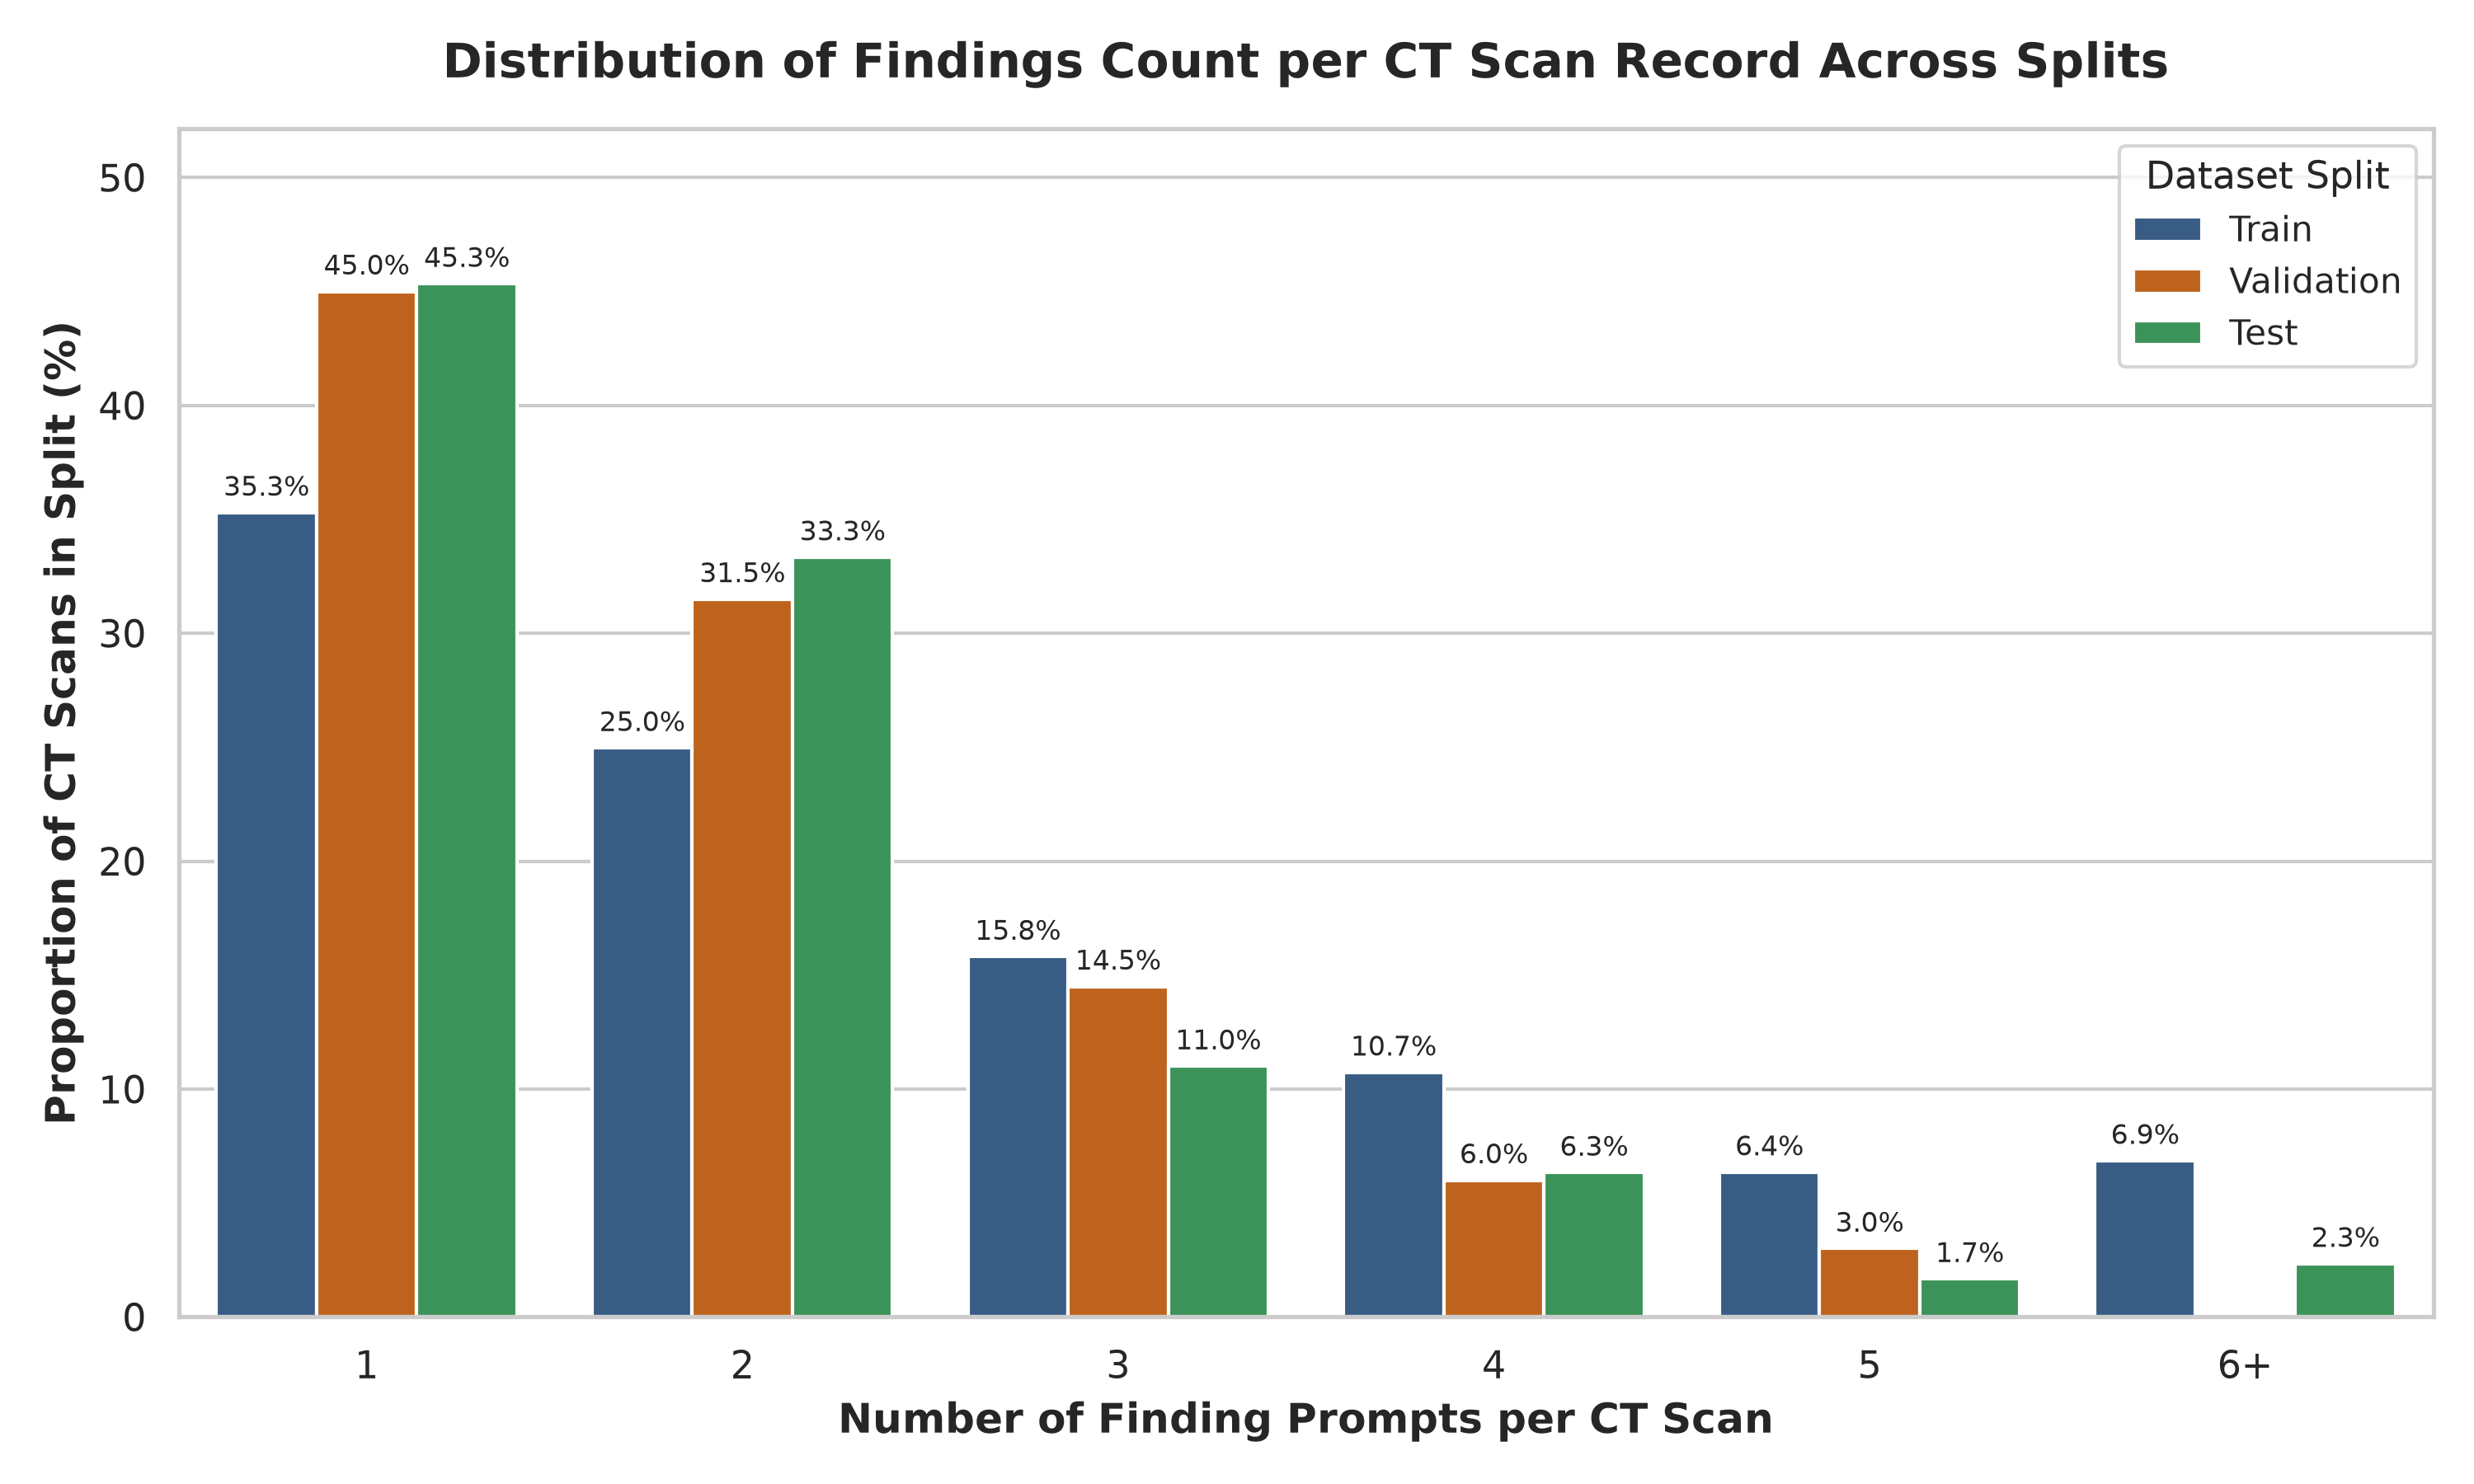
\includegraphics[width=\textwidth, height=0.68\textheight, keepaspectratio]{fig/exp001_findings_per_scan.png}
            \captionof{figure}{Findings per CT scan proportion (\%).}
        \end{column}
    \end{columns}
\end{frame}

% ==============================================================================
% SLIDE 6: Figure 2 - Connected Component Disparity
% ==============================================================================
\begin{frame}{Figure 2: Connected Component Instance Disparity}
    \begin{center}
        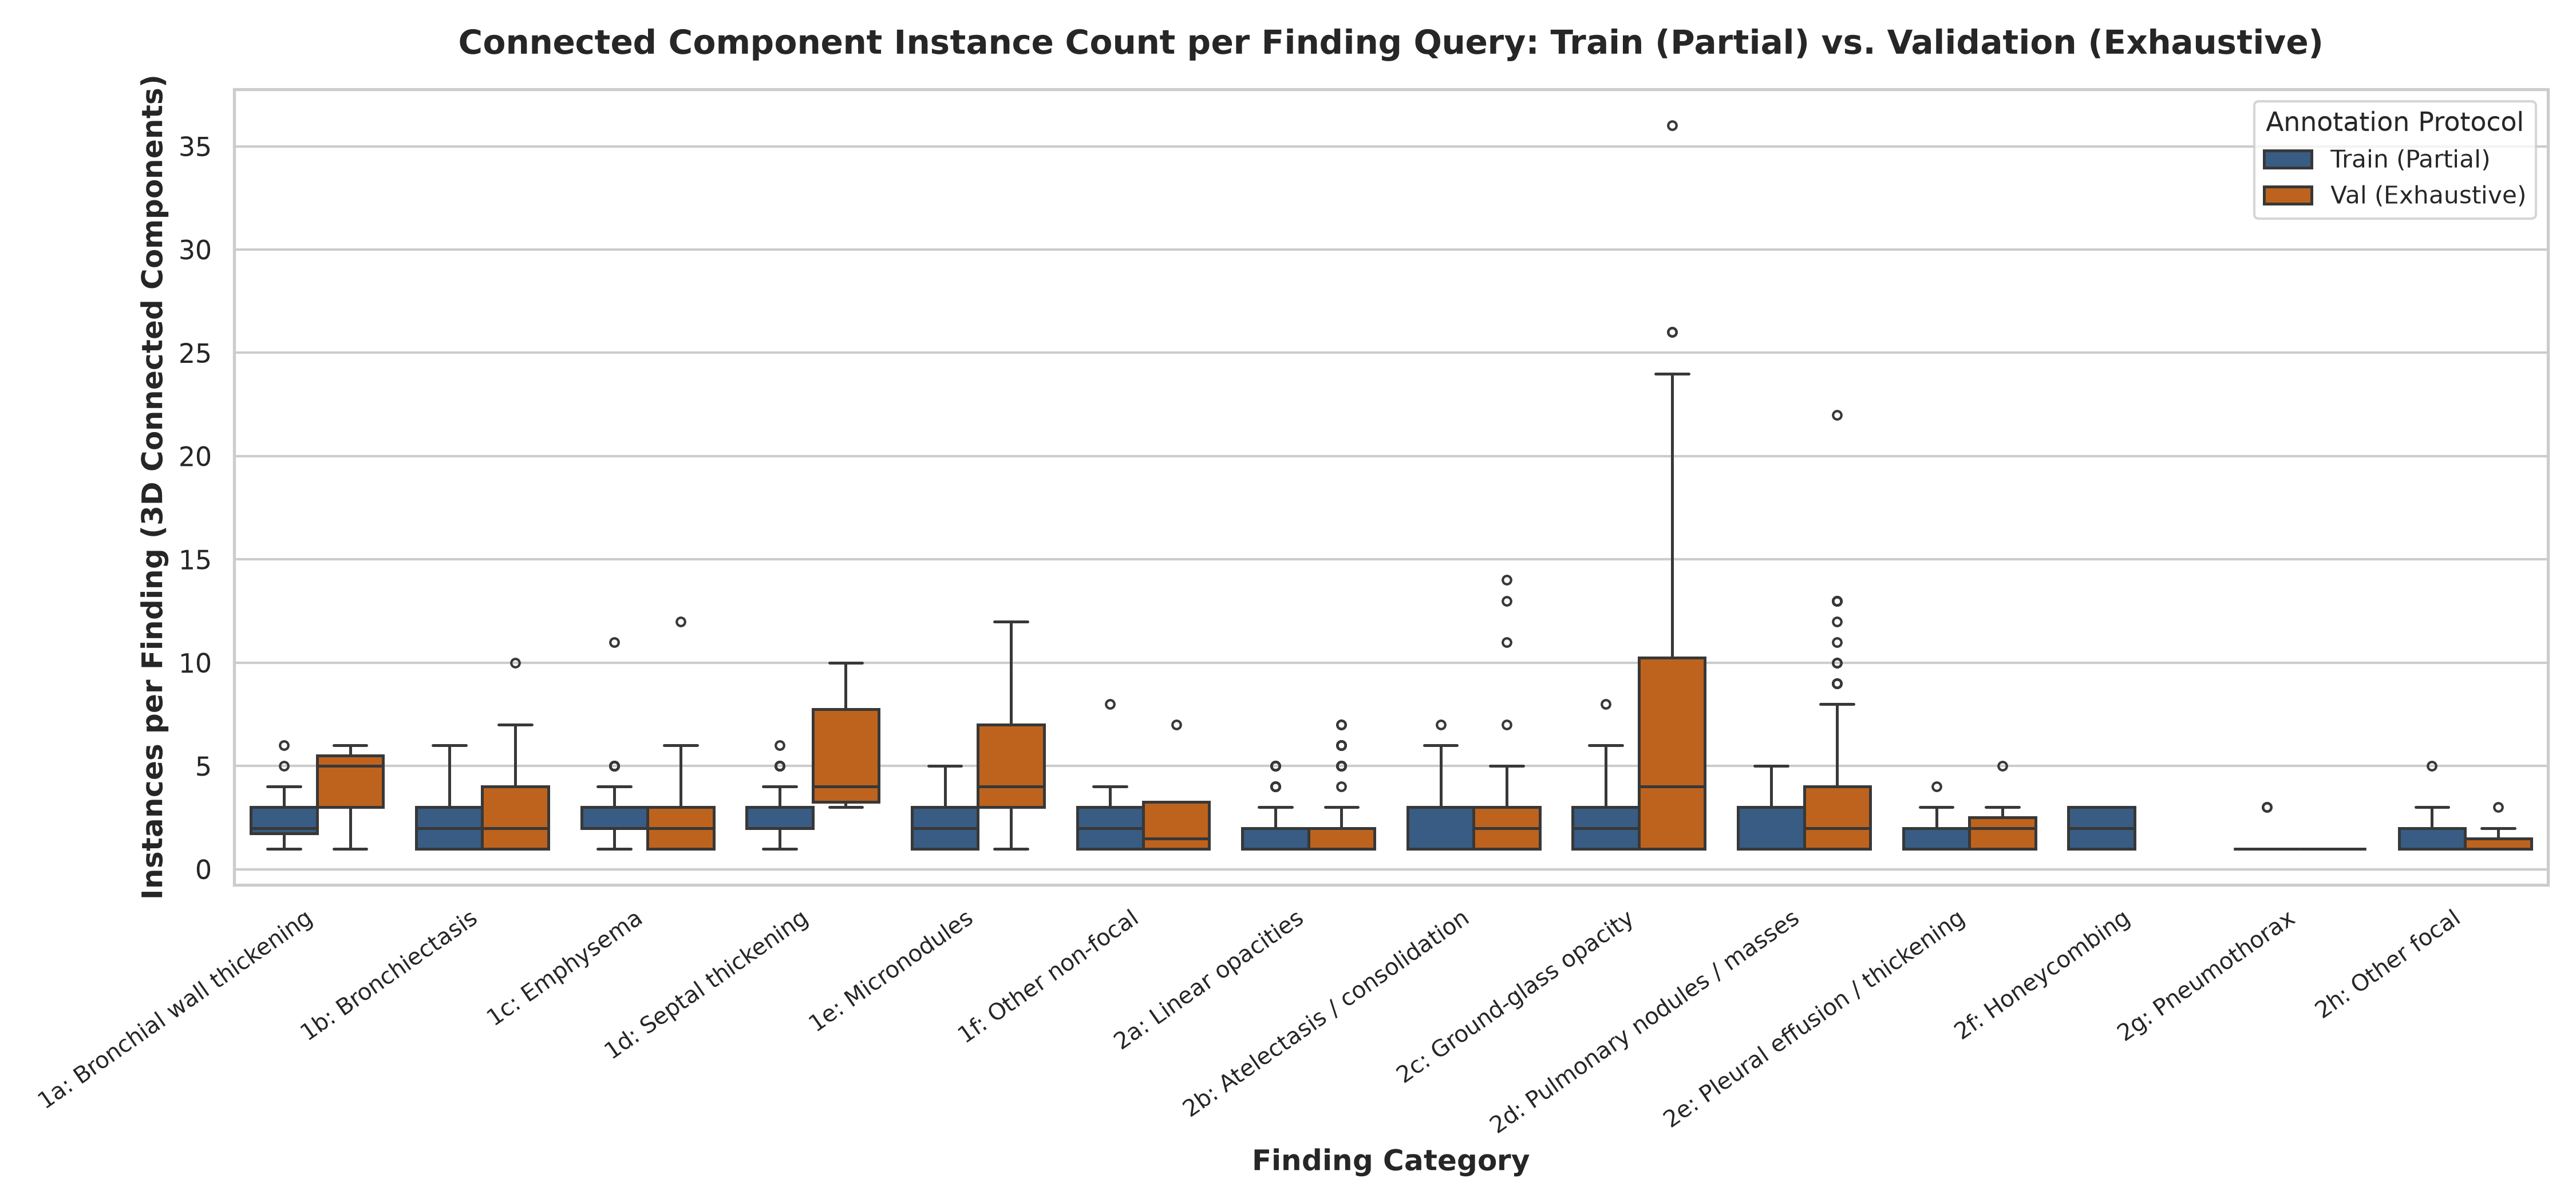
\includegraphics[width=0.88\textwidth, height=0.72\textheight, keepaspectratio]{fig/exp001_instance_count_boxplot.png}
    \end{center}
    \vspace{-0.5em}
    \captionof{figure}{Train (sparse $\le 3$) vs. Validation (exhaustive) instance counts per finding query.}
\end{frame}

% ==============================================================================
% SLIDE 7: Figure 3 - Co-Occurrence Matrix
% ==============================================================================
\begin{frame}{Figure 3: Multi-Finding Pathology Co-Occurrence}
    \begin{center}
        
\includegraphics[width=0.75\textwidth, height=0.75\textheight, keepaspectratio]{fig/exp001_cooccurrence_heatmap.png}
    \end{center}
    \vspace{-0.5em}
    \captionof{figure}{Scan-level conditional co-occurrence probability matrix $P(c_j \text{ present} \mid c_i \text{ present})$.}
\end{frame}

% ==============================================================================
% SLIDE 8: Table 3 - NLP Syntax Shift
% ==============================================================================
\begin{frame}{Table 3: Validation Prompt Text Shift (Cases 1--50 vs. 51--200)}
    \centering
    \small
    \begin{tabular}{lcccc}
        \toprule
        \textbf{Metric / Parameter} & \textbf{Cases 1--50 (Paper)} & \textbf{Cases 51--200 (MICCAI)} & \textbf{Ratio} & \textbf{\% Change} \\
        \midrule
        Total Finding Prompts & 115 & 266 & 2.31x & +131.3\% \\
        Total Word Tokens & 1,263 & 3,193 & 2.53x & +152.8\% \\
        Mean Word Count (words) & 10.98 & 12.00 & 1.09x & +9.3\% \\
        \rowcolor{blue!10}
        Max Word Count (words) & 21 & \textbf{35} & \textbf{1.67x} & \textbf{+66.7\%} \\
        Mean Character Length & 70.0 & 80.0 & 1.14x & +14.3\% \\
        \rowcolor{blue!10}
        Prompts with Comma Punctuation & 11.30\% & \textbf{23.68\%} & \textbf{2.10x} & \textbf{+12.38\% pt} \\
        Log-Normal TTR (1000 Tokens) & 0.1740 & 0.1651 & 0.95x & -5.11\% \\
        \bottomrule
    \end{tabular}

    \vspace{1em}
    \begin{itemize}
        \item \textbf{Key Takeaway:} $0.0\%$ subword context truncation ($<128$ tokens); hedging noise is negligible ($0.38\%$).
    \end{itemize}
\end{frame}

% ==============================================================================
% SLIDE 9: Table 4 - Spatial Centroids & 4-Tier Taxonomy
% ==============================================================================
\begin{frame}{Table 4: Canonical 3D RAS Centroids \& Spatial Taxonomy}
    \centering
    \tiny
    \setlength{\tabcolsep}{5pt}
    \begin{tabular}{clccc>{\bfseries}l}
        \toprule
        \textbf{Code} & \textbf{Finding Category} & \textbf{Train Centroid $(\text{RL}, \text{AP}, \text{IS})$} & $\Delta d$ & $S_{\text{cos}}$ & Spatial Taxonomy \\
        \midrule
        \texttt{1a} & Bronchial wall thickening & $(0.508, 0.439, 0.541)$ & 0.0825 & 0.0412 & Hilar / Peribronchial \\
        \texttt{1b} & Bronchiectasis           & $(0.510, 0.449, 0.545)$ & 0.0563 & 0.2059 & Hilar / Peribronchial \\
        \texttt{1c} & Emphysema                & $(0.504, 0.442, 0.667)$ & 0.1566 & 0.1756 & Apical Dominant \\
        \texttt{1d} & Septal thickening        & $(0.519, 0.420, 0.563)$ & 0.1092 & 0.2228 & Isotropic / Parenchymal \\
        \texttt{1e} & Micronodules             & $(0.517, 0.422, 0.537)$ & 0.1007 & 0.1111 & Isotropic / Parenchymal \\
        \texttt{1f} & Other non-focal          & $(0.501, 0.426, 0.545)$ & 0.1327 & 0.0671 & Isotropic / Parenchymal \\
        \texttt{2a} & Linear opacities         & $(0.474, 0.500, 0.535)$ & 0.0886 & 0.2562 & Isotropic / Parenchymal \\
        \texttt{2b} & Atelectasis / consolid.  & $(0.503, 0.433, 0.491)$ & 0.1084 & 0.3275 & Basal / Dependent \\
        \texttt{2c} & Ground-glass opacity     & $(0.510, 0.407, 0.519)$ & 0.1711 & 0.4432 & Isotropic / Parenchymal \\
        \texttt{2d} & Pulmonary nodules/masses & $(0.540, 0.452, 0.556)$ & 0.1012 & 0.0268 & Isotropic / Parenchymal \\
        \texttt{2e} & Pleural effusion/thick.  & $(0.535, 0.314, 0.484)$ & 0.2426 & 0.5032 & Basal / Dependent \\
        \texttt{2f} & Honeycombing             & $(0.457, 0.482, 0.498)$ & -- & -- & Basal / Dependent \\
        \texttt{2g} & Pneumothorax             & $(0.497, 0.516, 0.522)$ & 0.2293 & 0.0717 & Isotropic / Parenchymal \\
        \texttt{2h} & Other focal              & $(0.521, 0.442, 0.536)$ & 0.0633 & 0.0101 & Isotropic / Parenchymal \\
        \bottomrule
    \end{tabular}
\end{frame}

% ==============================================================================
% SLIDE 10: Figure 4 - 3D Spatial Probability Density Priors
% ==============================================================================
\begin{frame}{Figure 4: 3D Population Spatial Probability Density Priors}
    \begin{center}
        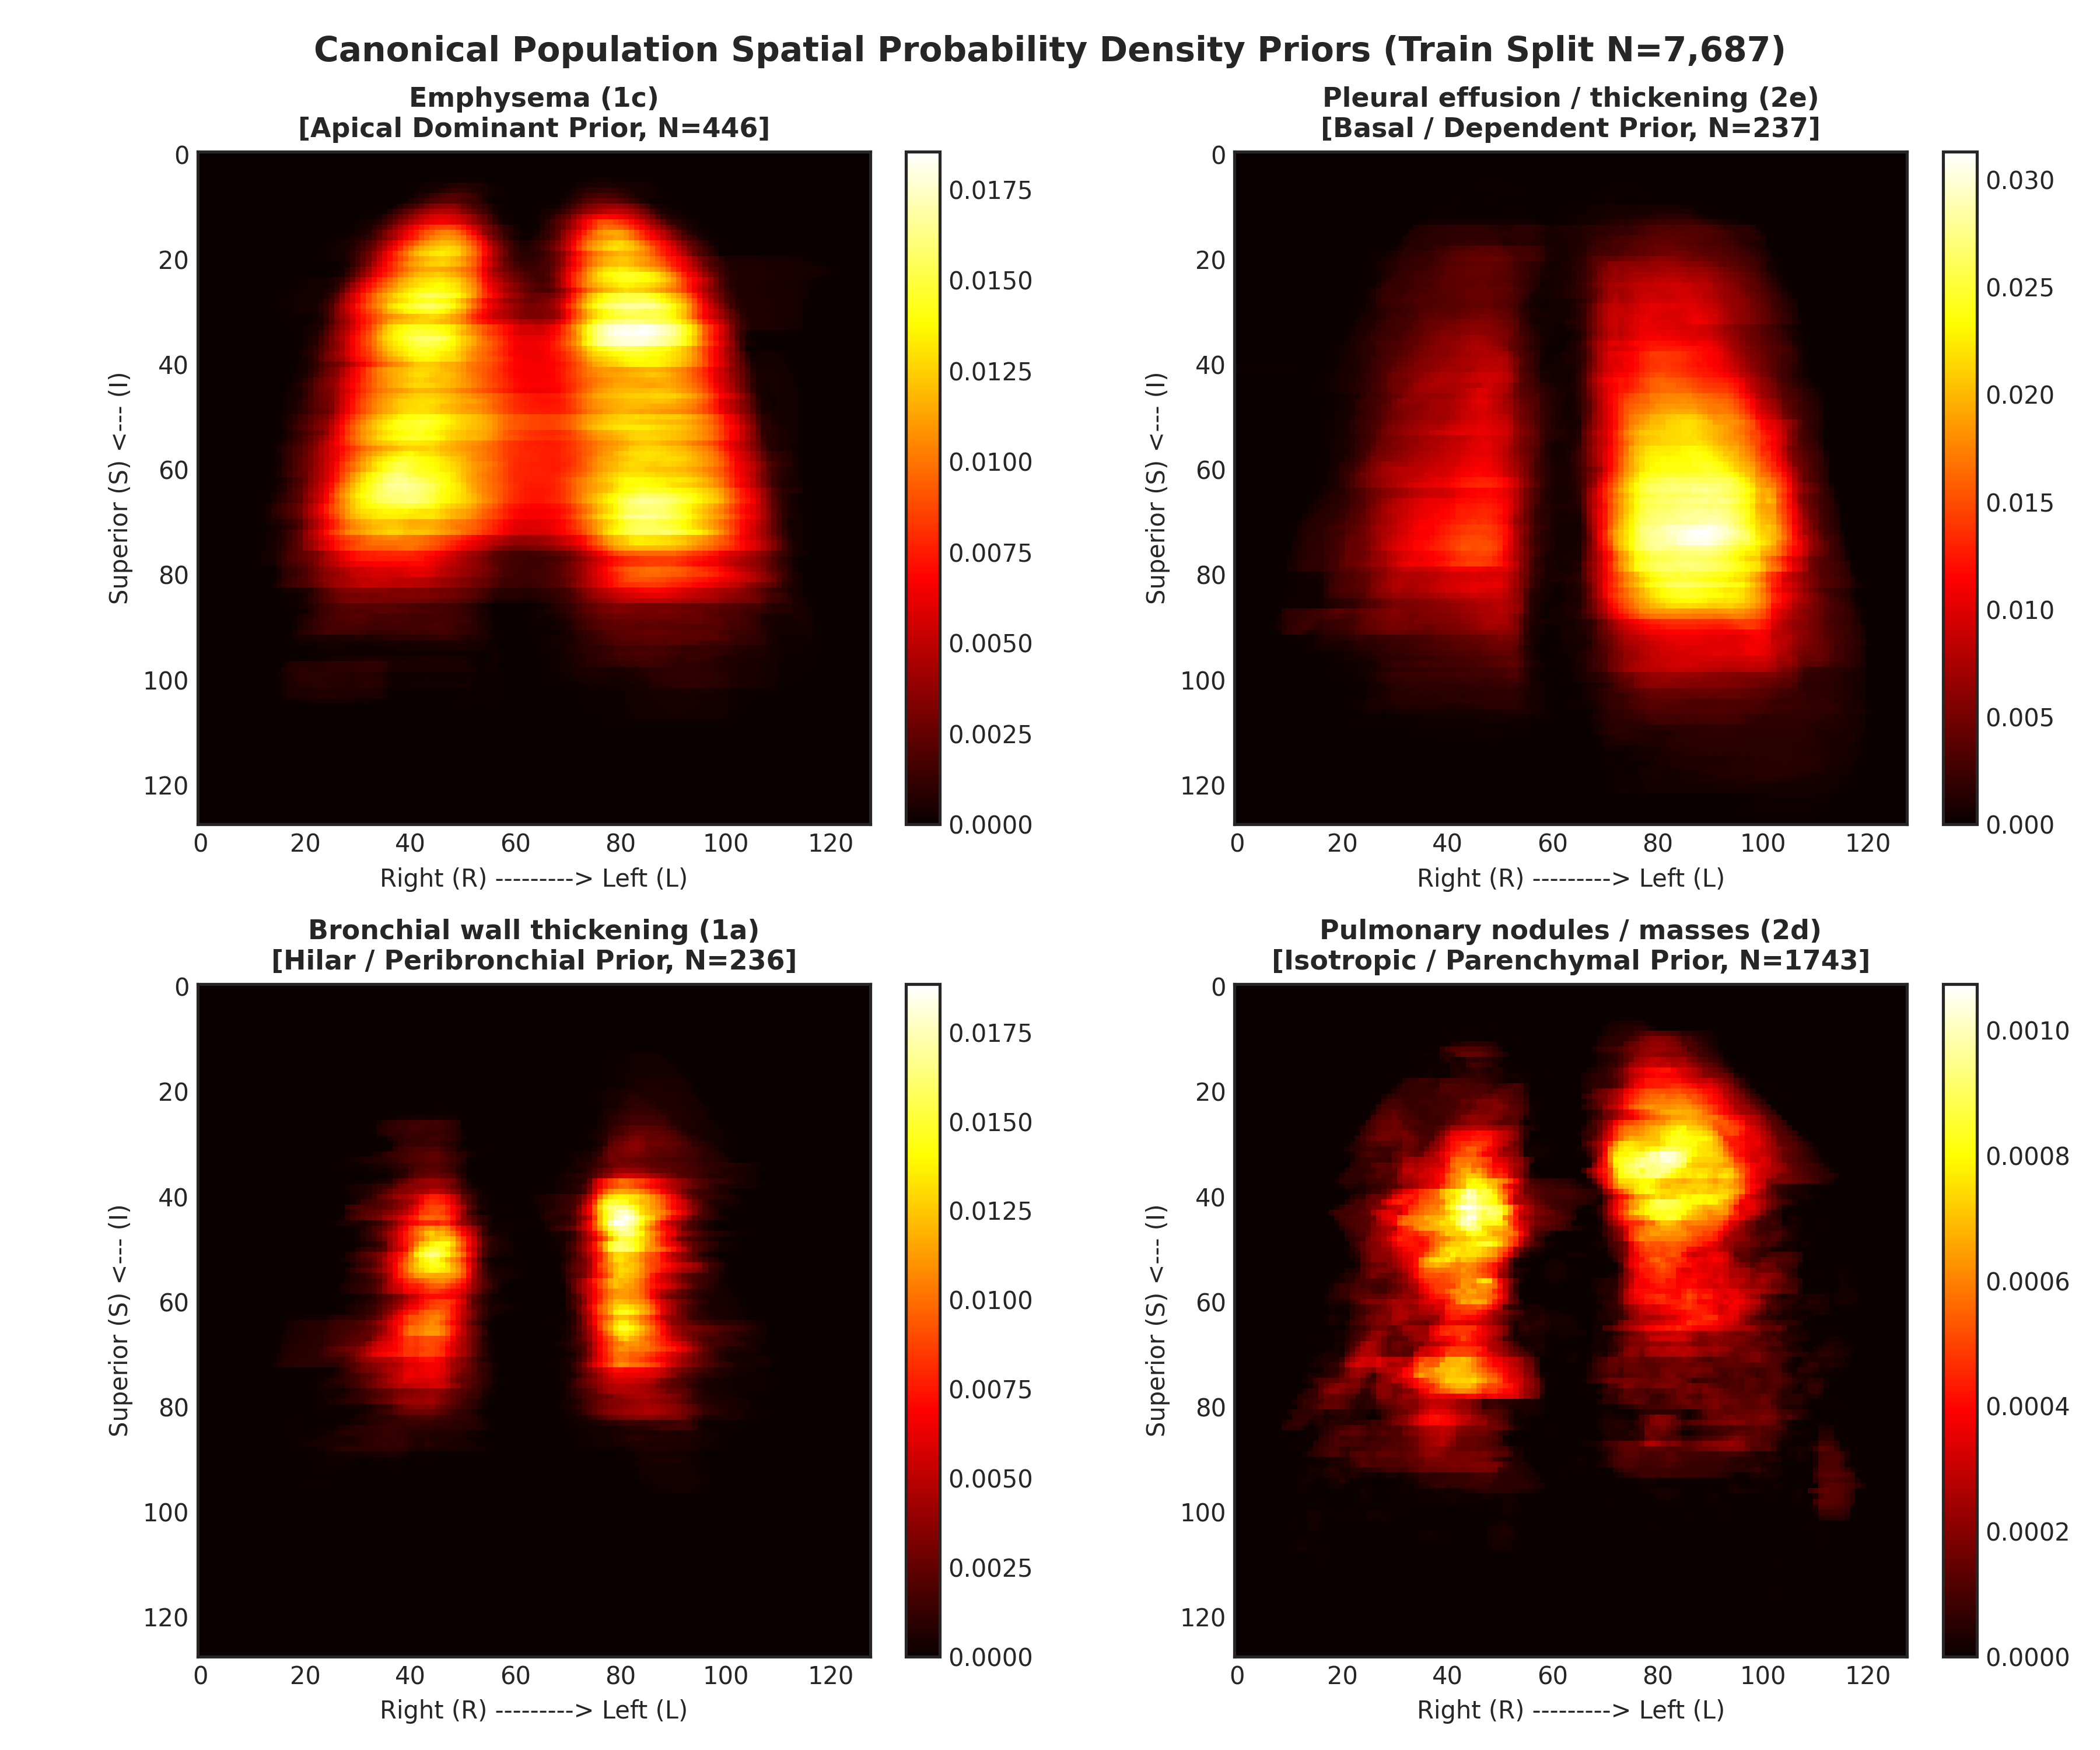
\includegraphics[width=0.82\textwidth, height=0.72\textheight, keepaspectratio]{fig/exp003_population_spatial_priors_4panel.png}
    \end{center}
    \vspace{-0.5em}
    \captionof{figure}{Coronal projections across Apical, Basal, Hilar, and Isotropic spatial taxonomies.}
\end{frame}

% ==============================================================================
% SLIDE 11: Table 5 - HU Attenuation & Intensity Bounds
% ==============================================================================
\begin{frame}{Table 5: Hounsfield Unit (HU) Attenuation Profiling}
    \centering
    \tiny
    \setlength{\tabcolsep}{6pt}
    \begin{tabular}{clcccc}
        \toprule
        \textbf{Code} & \textbf{Category Name} & \textbf{$N_{\text{masks}}$} & \textbf{Mean HU} & \textbf{Contrast $\Delta \text{HU}$} & \textbf{Rec Window [P5, P95] HU} \\
        \midrule
        \texttt{1a} & Bronchial wall thickening & 239 & -486.35 & -21.98 & [-933.0, +69.0] \\
        \texttt{1b} & Bronchiectasis           & 293 & -477.93 & +1.93  & [-934.0, +86.0] \\
        \texttt{1c} & Emphysema                & 463 & -307.95 & -3.11  & [-992.0, +251.0] \\
        \texttt{1d} & Septal thickening        & 200 & -406.38 & -21.23 & [-1001.0, +121.0] \\
        \texttt{1e} & Micronodules             & 325 & -427.36 & +15.16 & [-998.0, +101.0] \\
        \texttt{1f} & Other non-focal          & 154 & -334.71 & -8.61  & [-987.0, +98.0] \\
        \texttt{2a} & Linear opacities         & 1,189 & -286.55 & +4.68 & [-992.0, +399.0] \\
        \texttt{2b} & Atelectasis / consolid.  & 1,416 & -341.35 & +2.43 & [-995.0, +129.0] \\
        \texttt{2c} & Ground-glass opacity     & 1,567 & -375.11 & -4.51 & [-995.0, +137.0] \\
        \texttt{2d} & Pulmonary nodules/masses & 1,875 & -427.06 & -49.15 & [-995.0, +194.0] \\
        \texttt{2e} & Pleural effusion/thick.  & 248 & -368.59 & -19.37 & [-1007.0, +135.0] \\
        \texttt{2f} & Honeycombing             & 16  & -420.45 & -18.07 & [-905.0, +83.0] \\
        \texttt{2g} & Pneumothorax             & 19  & -306.85 & -54.68 & [-961.0, +148.0] \\
        \texttt{2h} & Other focal              & 64  & -156.62 & -16.21 & [-915.0, +201.0] \\
        \bottomrule
    \end{tabular}
\end{frame}

% ==============================================================================
% SLIDE 12: Figure 5 - HU Violins & Contrast Deltas
% ==============================================================================
\begin{frame}{Figure 5: HU Radiodensity \& Contrast Deltas}
    \begin{columns}[c]
        \begin{column}{0.5\textwidth}
            \centering
            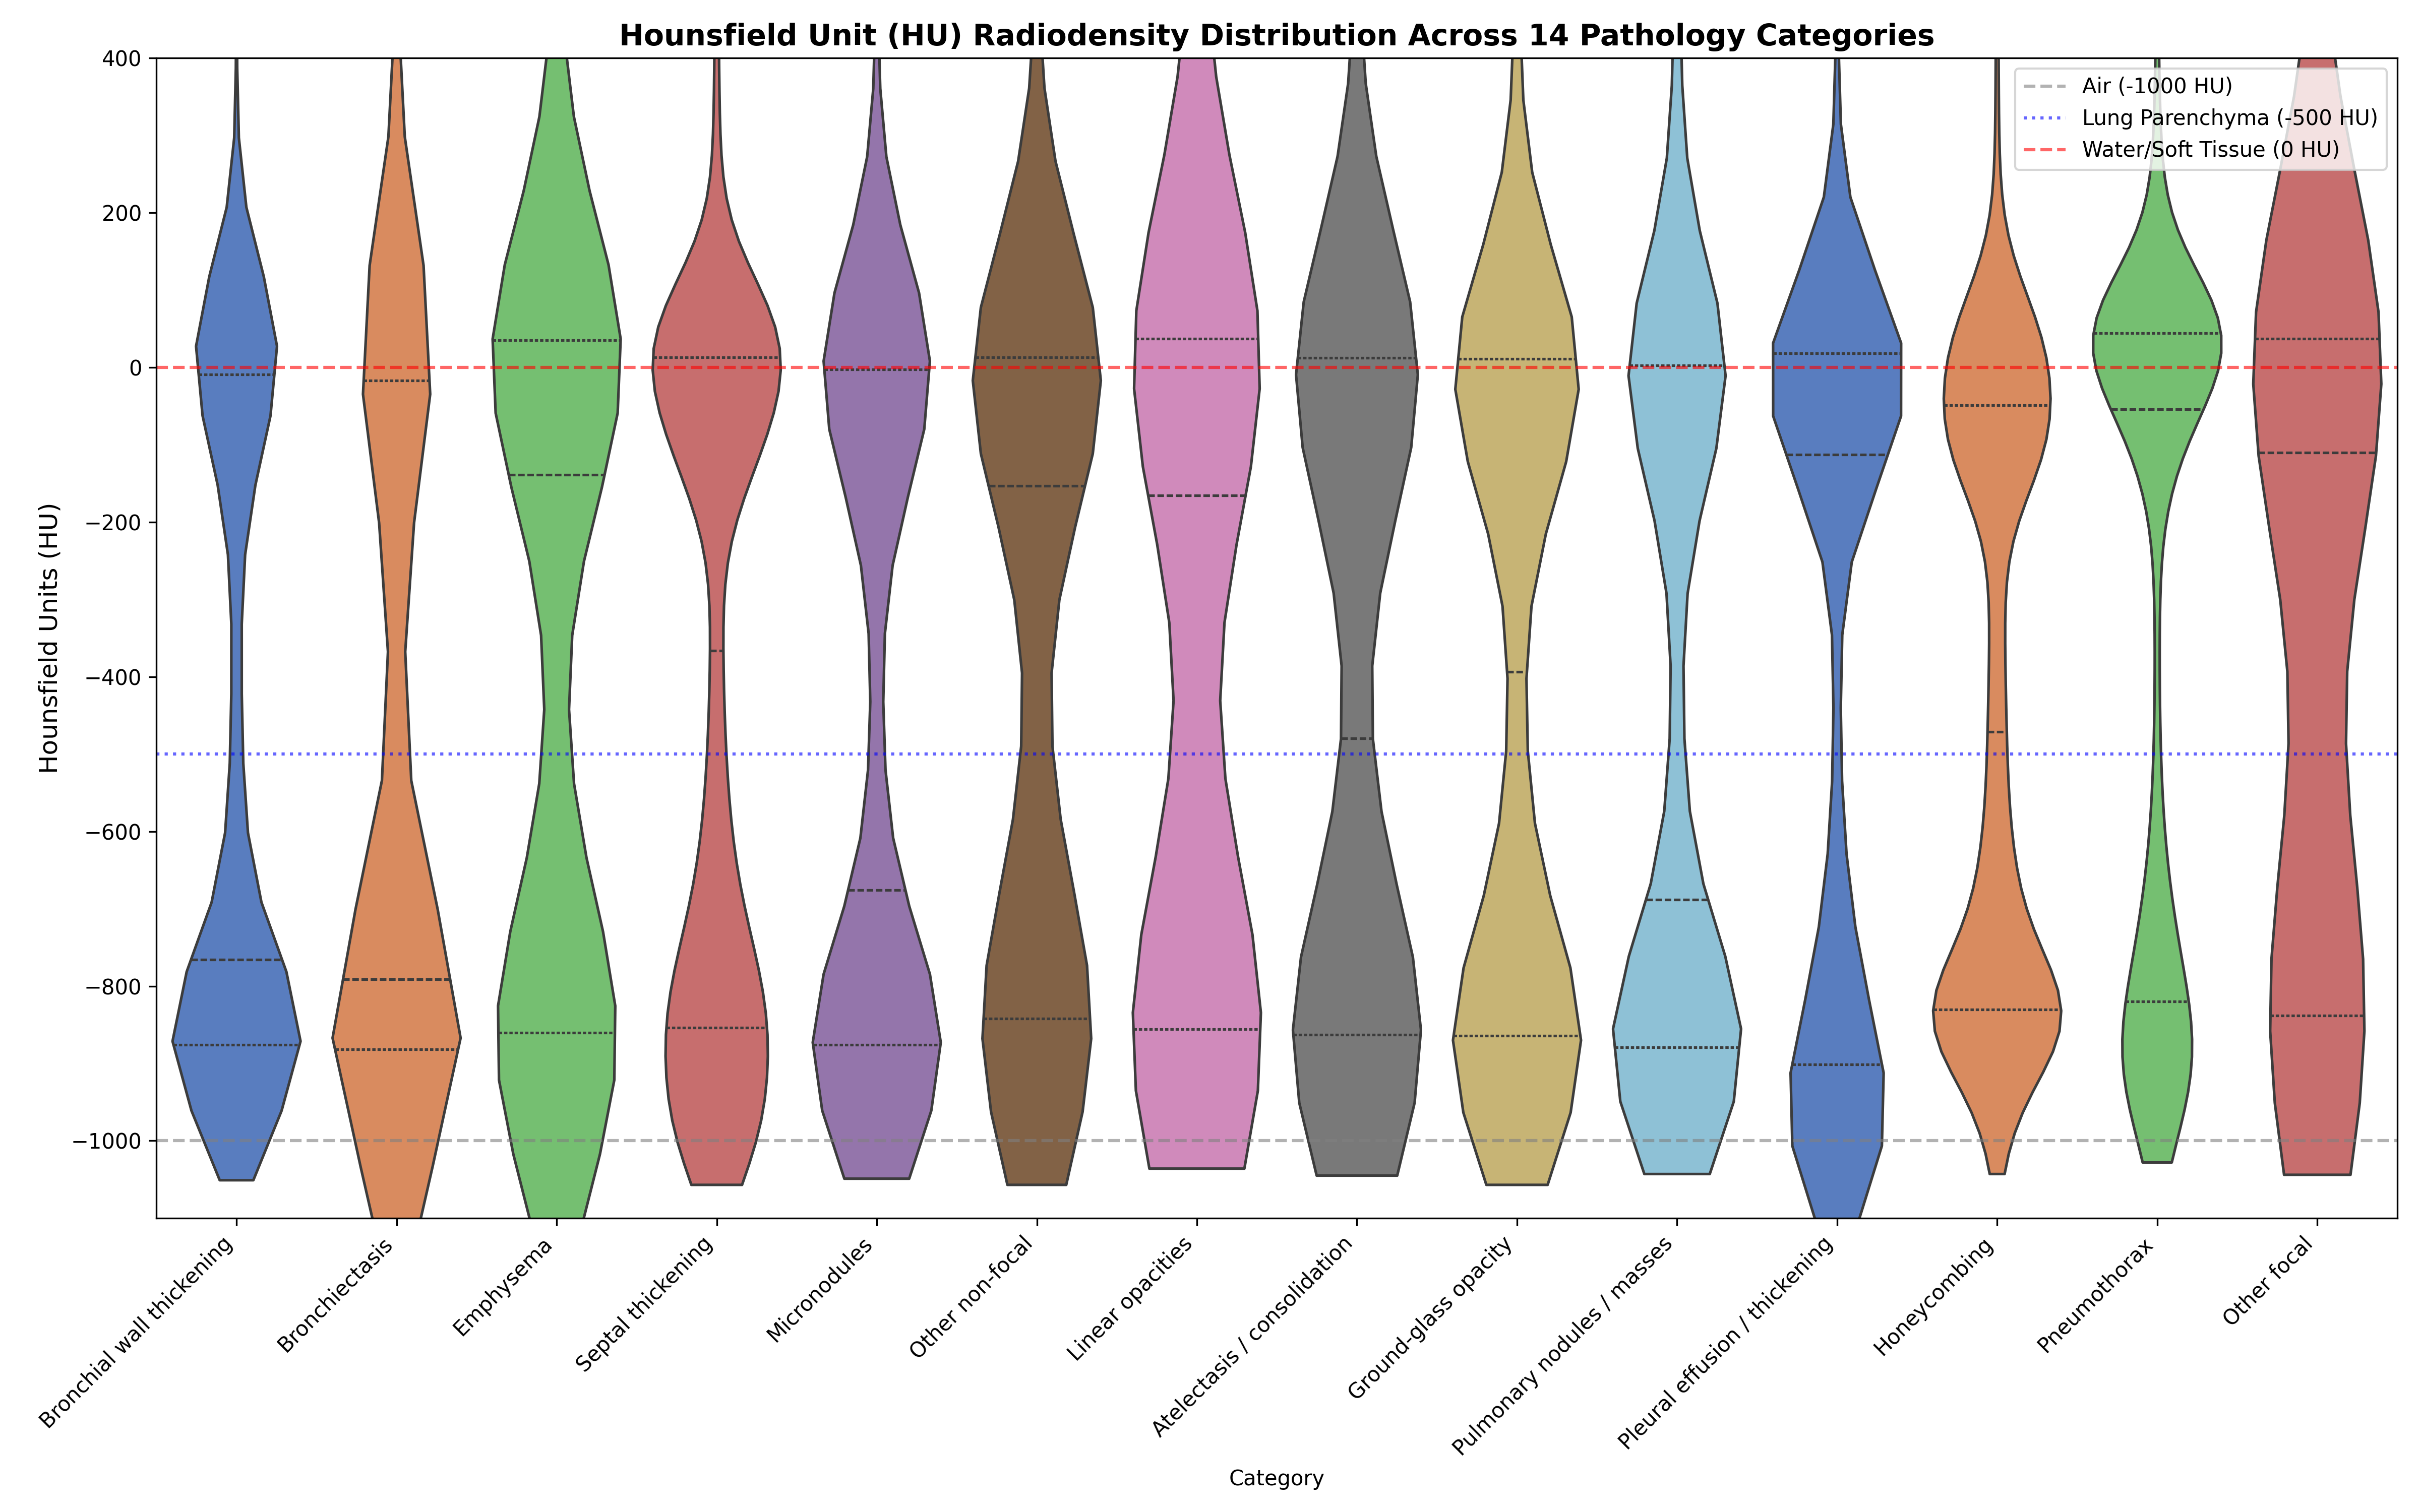
\includegraphics[width=\textwidth, height=0.68\textheight, keepaspectratio]{fig/exp004_hu_distribution_violin.png}
            \captionof{figure}{HU radiodensity violin distributions.}
        \end{column}
        \begin{column}{0.5\textwidth}
            \centering
            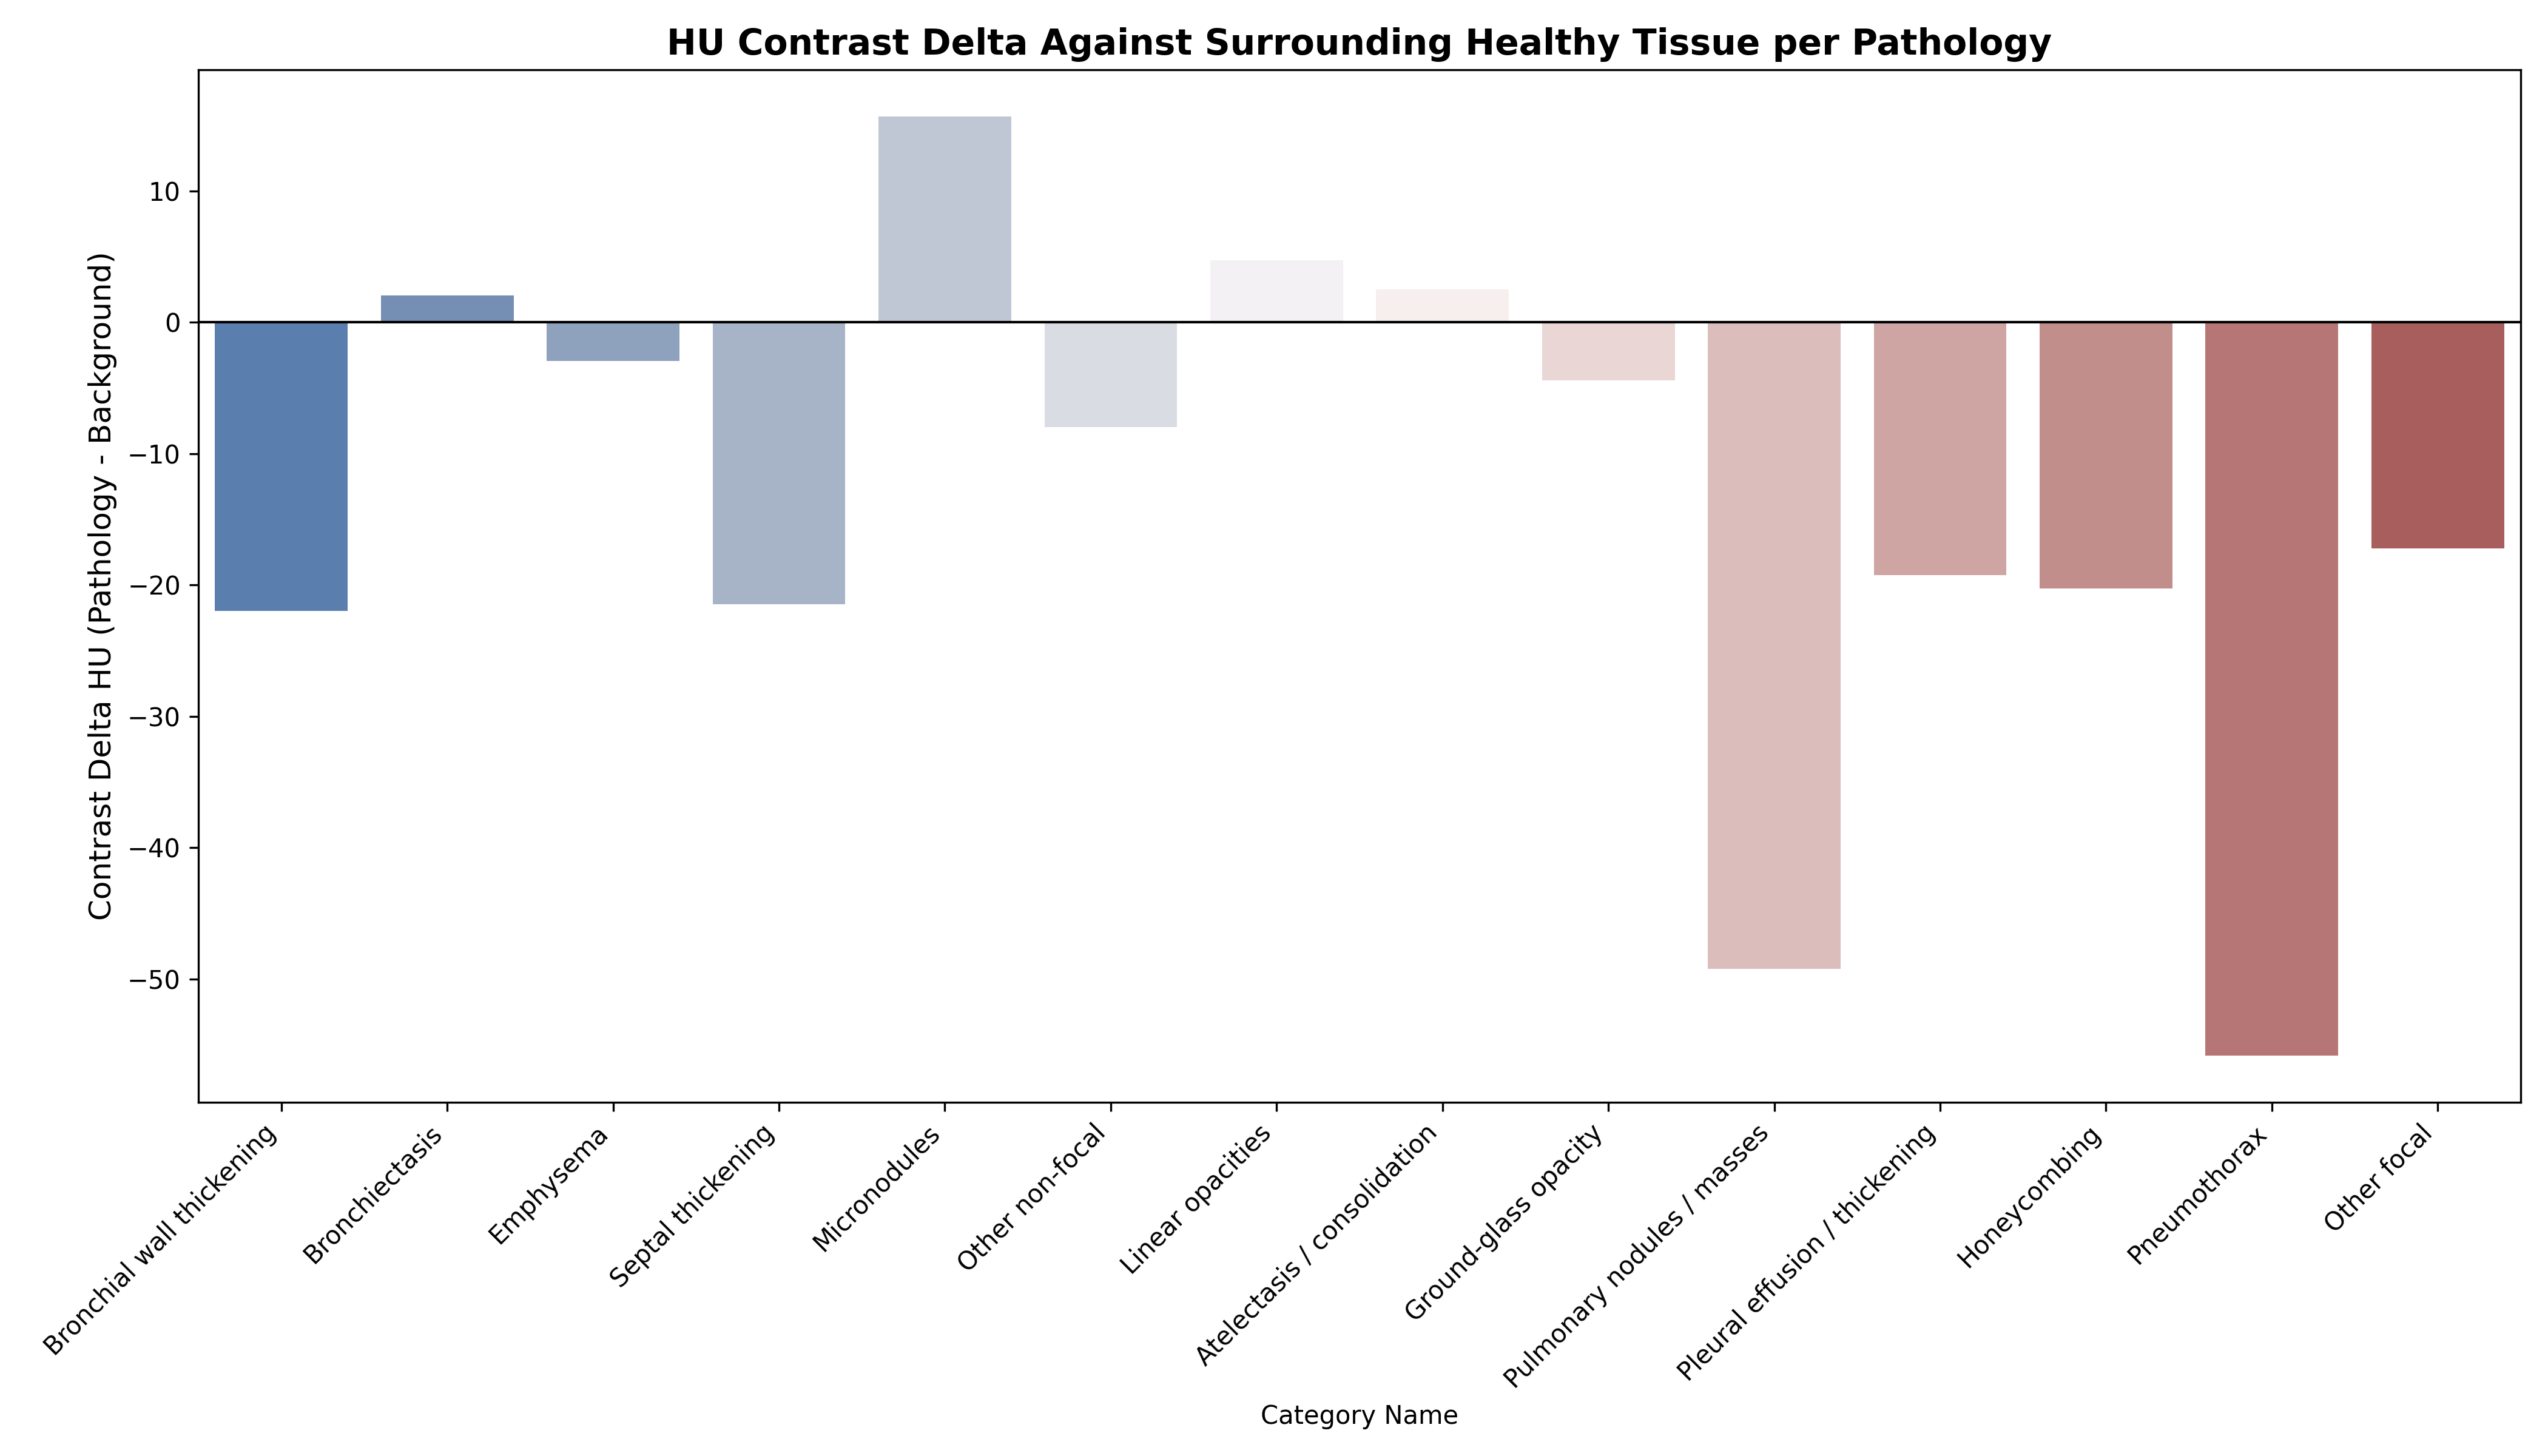
\includegraphics[width=\textwidth, height=0.68\textheight, keepaspectratio]{fig/exp004_hu_contrast_delta_barplot.png}
            \captionof{figure}{Contrast delta $\Delta \text{HU}$ (Pathology vs. Bg).}
        \end{column}
    \end{columns}
\end{frame}

% ==============================================================================
% SLIDE 13: Table 6 - Morphological Topology & Noise Pruning
% ==============================================================================
\begin{frame}{Table 6: 3D Connected Component Topology \& Pruning}
    \centering
    \tiny
    \setlength{\tabcolsep}{4pt}
    \begin{tabular}{clccccc>{\bfseries}c}
        \toprule
        \textbf{Code} & \textbf{Category Name} & \textbf{Blobs} & \textbf{Blobs/Find} & \textbf{Sphericity ($S$)} & \textbf{Median Vol ($\text{mm}^3$)} & \textbf{P95 Vol ($\text{mm}^3$)} & Rec Min Size \\
        \midrule
        \texttt{1a} & Bronchial wall thickening & 1,539 & 6.44 & 0.7249 & 90.0 & 88,920.0 & 10 voxels \\
        \texttt{1b} & Bronchiectasis           & 1,007 & 3.44 & 0.6063 & 1,453.0 & 185,597.3 & 10 voxels \\
        \texttt{1c} & Emphysema                & 2,279 & 4.92 & 0.7155 & 578.0 & 193,390.3 & 10 voxels \\
        \texttt{1d} & Septal thickening        & 726 & 3.63 & 0.5434 & 2,844.5 & 197,179.8 & 10 voxels \\
        \texttt{1e} & Micronodules             & 1,210 & 3.72 & 0.7502 & 236.0 & 148,146.1 & 10 voxels \\
        \rowcolor{blue!10}
        \texttt{1f} & Other non-focal          & 469 & 3.05 & 0.6177 & 2,664.0 & 305,819.8 & \textbf{47 voxels} \\
        \texttt{2a} & Linear opacities         & 3,248 & 2.73 & 0.6141 & 1,402.0 & 34,399.5 & 10 voxels \\
        \texttt{2b} & Atelectasis / consolid.  & 5,662 & 4.00 & 0.6453 & 943.0 & 126,002.1 & 10 voxels \\
        \texttt{2c} & Ground-glass opacity     & 6,080 & 3.88 & 0.6638 & 1,942.5 & 152,727.0 & 10 voxels \\
        \rowcolor{blue!10}
        \texttt{2d} & Pulmonary nodules/masses & 3,836 & 2.05 & \textbf{0.9416} & 192.0 & 3,204.0 & \textbf{15 voxels} \\
        \texttt{2e} & Pleural effusion/thick.  & 749 & 3.02 & 0.5712 & 1,863.0 & 602,883.4 & 10 voxels \\
        \texttt{2f} & Honeycombing             & 55  & 3.44 & 0.6378 & 4,990.0 & 189,603.9 & 10 voxels \\
        \texttt{2g} & Pneumothorax             & 84  & 4.42 & 0.6807 & 42.0 & 261,443.2 & 10 voxels \\
        \texttt{2h} & Other focal              & 194 & 3.03 & 0.6434 & 1,245.0 & 225,928.0 & 10 voxels \\
        \bottomrule
    \end{tabular}
\end{frame}

% ==============================================================================
% SLIDE 14: Actionable Directives
% ==============================================================================
\begin{frame}{Calibrated Actionable Modeling Directives}
    \begin{columns}[c]
        \begin{column}{0.95\textwidth}
            \begin{enumerate}
                \item \textbf{PU Loss Formulation:} PU-SPOCO + Multi-Planar Reconstruction (MPR) consistency loss to handle training label caps ($\le 3$ instances).
                \item \textbf{Category Intensity Windowing:} Preprocess CT volumes using category HU bounds \texttt{[min\_HU, max\_HU]} (Exp 004).
                \item \textbf{Spatial Prior Masking:} Apply 3D RAS spatial probability density priors $P(\mathbf{x}' \in \text{mask} \mid c)$ to bound search space (Exp 003).
                \item \textbf{Component Noise Pruning:} Filter binarized predictions with \texttt{recommended\_min\_size\_voxels} thresholds (Exp 005).
                \item \textbf{4D Back-Reorientation:} Re-orient predictions via parent CT affine matrices prior to evaluation.
            \end{enumerate}
        \end{column}
    \end{columns}
\end{frame}

\end{document}